\documentclass[12pt]{beamer}
\usetheme{Warsaw}
\usepackage[utf8]{inputenc}
\usepackage[english]{babel}
\usepackage{amsmath}
\usepackage{stmaryrd}
\usepackage{amsfonts}
\usepackage{amssymb}
\usepackage{graphicx}
\usepackage{xcolor}
\usepackage[backend=bibtex, style=authoryear, maxcitenames=2]{biblatex}
\addbibresource{../../Thesis/references.bib} 
\renewcommand*{\bibfont}{\footnotesize}
\usepackage{url}
\definecolor{lila}{RGB}{128,0,128}

\newcommand{\myCite}[1]{{\scriptsize\parencite{#1}}}

\setbeamertemplate{navigation symbols}{}
\setbeamertemplate{footline}{%
	\raisebox{5pt}{%
		\makebox[\paperwidth]{%
			\hfill\makebox[10pt]{%
				\textcolor{gray}{\footnotesize\insertframenumber}
			}
		}
	}
}

\definecolor{regal}{RGB}{81,0,0}
\usepackage{array}
\usepackage{colortbl}
\makeatletter
\newcommand{\thickhline}{%
    \noalign {\ifnum 0=`}\fi \color{regal}\hrule height 4pt
    \futurelet \reserved@a \@xhline
}
\newcolumntype{"}{@{\color{regal}\hskip\tabcolsep\vrule width 8pt\hskip\tabcolsep}}
\makeatother

% listings
\usepackage[TS1,T1]{fontenc}
\usepackage{newunicodechar}
\newcommand*\longs{{\fontencoding{TS1}\selectfont s}}
\newunicodechar{ſ}{\longs}
\usepackage{listings}
\lstset{
	captionpos=b,
	frame=single,
	breaklines=true,
	tabsize=2,
	aboveskip=4pt,
	belowskip=6pt,
	literate=%
		{Ö}{{\"O}}1
		{Ä}{{\"A}}1
		{Ü}{{\"U}}1
		{ß}{{\ss}}1
		{ü}{{\"u}}1
		{ä}{{\"a}}1
		{ö}{{\"o}}1
		{~}{{\textasciitilde}}1,
	alsoletter={{\"u}}
}
\definecolor{maroon}{rgb}{0.5,0,0}
\definecolor{darkgreen}{rgb}{0,0.5,0}
\lstdefinelanguage{XML}
{
	basicstyle=\ttfamily\tiny,
	morestring=[s]{"}{"},
	morecomment=[s]{?}{?},
	morecomment=[s]{!--}{--},
	commentstyle=\color{darkgreen},
	moredelim=[s][\color{black}]{>}{<},
	moredelim=[s][\color{red}]{\ }{=},
	stringstyle=\color{blue},
	identifierstyle=\color{maroon}
}

%\setbeamercovered{transparent} 
%\logo{}  
%\subject{} 
\begin{document} 
		
\begin{frame}[plain,noframenumbering]
	\begin{minipage}{0.1\textwidth}
		\hspace{-0.5cm}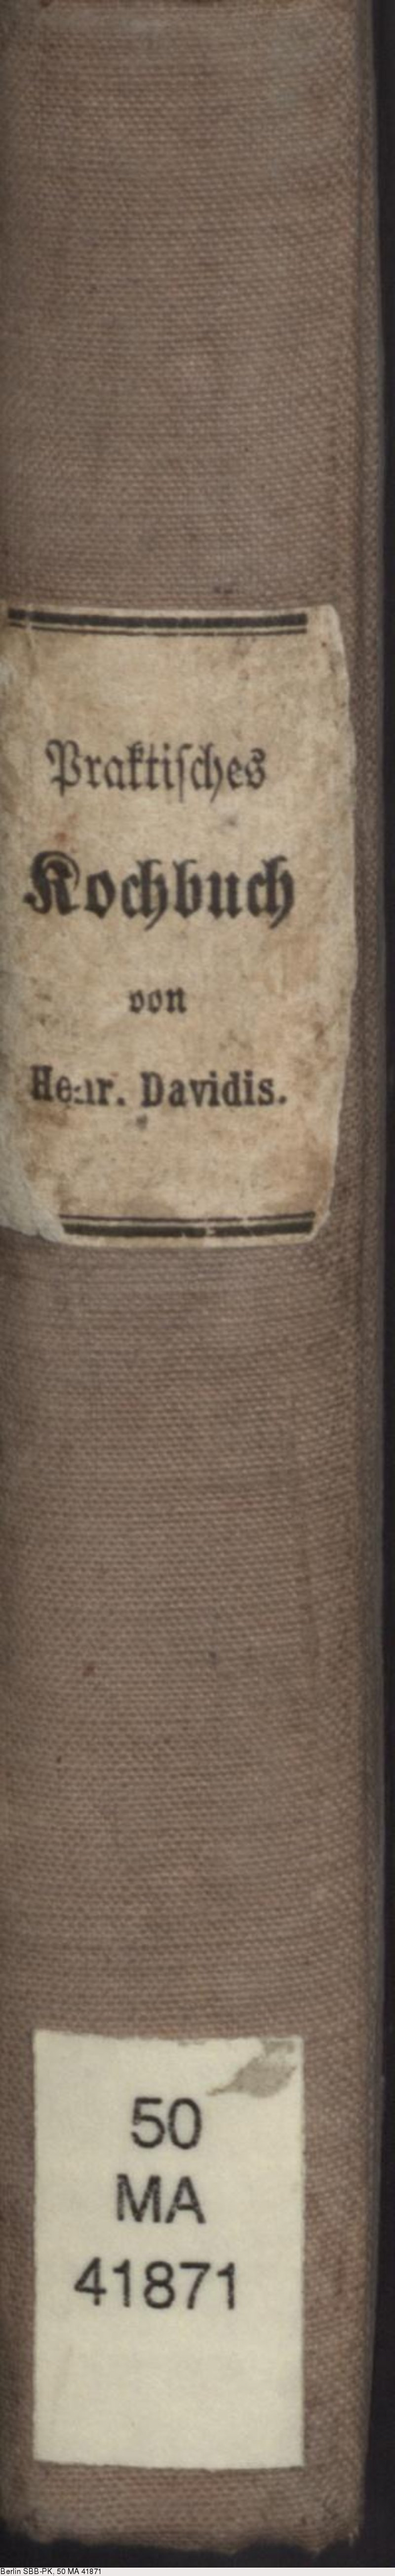
\includegraphics[scale=0.049]{Images/Buchruecken}
	\end{minipage}
	\begin{minipage}{0.6\textwidth}
		\begin{center}
			\vspace{-1.5cm}
			\Large{Extracting recipe ingredients \\ from cookbooks} \\
			\vspace{0.5cm}
			\large{Related Work} \\
			\small{von \\ \vspace{-0.1cm} Torsten Knauf}
		\end{center}
	\end{minipage}
	\begin{minipage}{0.25\textwidth}
		\arrayrulecolor{red}
		\small
		\begin{tabular}{"l}
			Der Beginn einer \\ Master-Arbeit \\
			\thickhline
			\color{white} \\
			\color{white} \\
			\thickhline 
			\color{white} - \\
			\color{white} - \\
			\thickhline 
			\color{white} - \\
			\color{white} - \\
			\thickhline 
			\color{white} - \\
			\color{white} - \\
			\thickhline 
			\color{white} - \\
			\color{white} - \\
			\thickhline 
			\color{white} - \\
			\color{white} - 
		\end{tabular}
	\end{minipage}
\end{frame}

\begin{frame}
	\tableofcontents
\end{frame}

\section{Tag-Schema}
\begin{frame}{}
	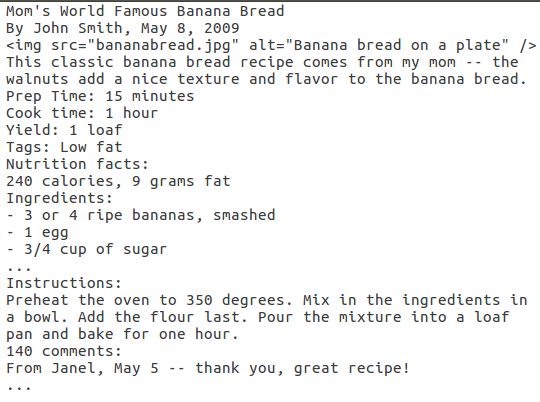
\includegraphics[width=0.7\textwidth]{Images/schemaRecipeWithoutMarkup} \\
	\myCite{schemaOrg}
\end{frame}
	
\begin{frame}{}
	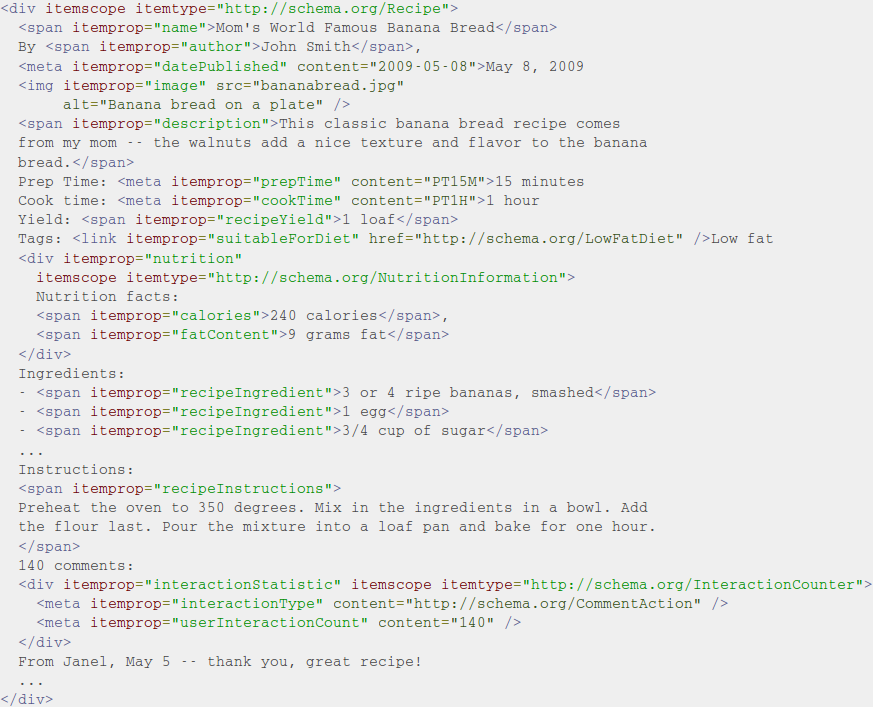
\includegraphics[width=0.95\textwidth]{Images/schemaRecipeWithMarkup} \\
	\myCite{schemaOrg}
\end{frame}

\begin{frame}{}
	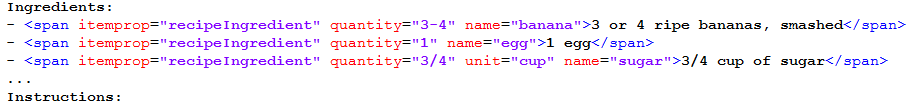
\includegraphics[width=1\textwidth]{Images/exampleCueML} \\
\end{frame}

\begin{frame}[fragile]
	\begin{lstlisting}[language=XML, caption={Beispiel Rezept von Frau Davidis}]
	<recipe type="Suppen." rcp-id="B-16">
		<head>Mock Turtle Suppe.</head>	
		
		<p>Es wird hierzu für 24-30 Personen eine kräftige Bouillon von 8-10 Pfund Rindfleisch mit Wurzelwerk gekocht. Zugleich bringt man einen großen Kalbskopf, eine Schweineschnauze und Ohren, einen Ochsengaumen und eine geräucherte Ochsenzunge zu Feuer und kocht dies Alles gahr, aber nicht zu weich. Kalt, schneidet man es in kleine, länglich viereckige Stückchen, gibt das Fleisch in die Bouillon, nebst braunem Gewürz, ein Paar Messerspitzen Cayenne-Pfeffer, einige Kalbsmidder in Stückchen geschnitten (siehe Vorbereitungsregeln), kleine Saucissen, so viel Kalbskopfbrühe, daß man hinreichend Suppe hat, und macht dies mit in Butter braun gemachtem Mehl gebunden. Nachdem dies Alles 1/4 Stunde gekocht hat, kommen noch Klöße von Kalbfleisch, einige hart gekochte Eier in Würfel geschnitten, ein Paar Eßlöffel Engl. Soja hinzu, und wenn die Klößchen einige Minuten gekocht haben, 1/2 Flasche Madeira und auch Austern, wenn man sie haben kann. Dann wird die Suppe sogleich angerichtet.</p>	
			
		<note>Anmerk. Der Soja macht die Suppe gewürzreicher, kann jedoch gut wegbleiben, und statt Madeira kann man weißen Franzwein und etwas Rum nehmen. Sowohl die Bouillon als Kalbskopf können schon am vorhergehenden Tage, ohne Nachtheil der Suppe, gekocht werden. </note>
	</cue:recipe>
	\end{lstlisting}
\end{frame}

\begin{frame}[fragile]
\begin{lstlisting}[language=XML, caption={Rezept mit cueML}]
<div itemscope itemtype="http://schema.org/Recipe http://cueML.org">
	<recipe type="Suppen." rcp-id="B-16">
		<head><span itemprop="name">Mock Turtle Suppe</span></head>
		
		<meta>
			<span itemprop="recipeYield" quantity="24-30" unit="Personen">24-30 Personen</span>
			<span itemprop="recipeIngredient" name="Bouillon" reference="#Bouillon">Bouillon</span>
			<span itemprop="recipeIngredient" name="Rindfleisch" quantity="8-10" unit="Pfund">8-10 Pfund Rindfleisch</span>
			<span itemprop="recipeIngredient">Wurzelwerk</span>
			<span itemprop="recipeIngredient" name="Cayennepfeffer" quantity="vague" unit="Messersptize">ein Paar Messerspitzen Cayenne-Pfeffer</span>
			<span itemprop="recipeIngredient" name="Ei" quantity="vague">einige hart gekochte Eier</span>
			...
			<span itemprop="recipeIngredient" name="Auster" isOptional="True">Austern, wenn man sie haben kann</span>
			<span itemprop="recipeIngredient" quantity="vague" unit="EL" isOptional="True">ein Paar Eßlöffel Engl. Soja</span>
			<recipeIngredientAlternations>
				<alt>
					<span itemprop="recipeIngredient" name="Madeira" quantity="0.5" unit="Flasche">Madeira</span>
				</alt>
				<alt>
					<span itemprop="recipeIngredient" name="weißen Franzwein">weißen Franzwein</span>
					<span itemprop="recipeIngredient" name="Rum" quantity="vague">etwas Rum</span>
				</alt>
			</recipeIngredientAlternations>
		</meta>
		<span itemprop="recipeInstructions">...</span>
	<recipe>
</div>		
\end{lstlisting}
\end{frame}

\begin{frame}[fragile]
\begin{lstlisting}[language=XML, caption={Rezept mit besserem cueML}]
<div itemscope itemtype="http://schema.org/Recipe http://cueML.org">
	<recipe type="Suppen." rcp-id="B-16">
		<meta>
			<span itemprop="name" content="Mock Turtle Suppe"/>
			
			<span itemprop="recipeYield" quantity="24-30" unit="Personen"/>
			
			<span itemprop="recipeIngredient" name="Bouillon" reference="#Bouillon"/>
			<span itemprop="recipeIngredient" name="Rindfleisch" quantity="8-10" unit="Pfund"/>
			<span itemprop="recipeIngredient" uncertainName="Wurzelwerk"/>
			<span itemprop="recipeIngredient" name="Cayennepfeffer" quantity="vague" unit="Messersptize"/>
			<span itemprop="recipeIngredient" name="Ei" quantity="vague"/>
			...
			<span itemprop="recipeIngredient" name="Auster" isOptional="True"/>
			<span itemprop="recipeIngredient" uncertainName="Engl. Soja" quantity="vague" unit="EL" isOptional="True"/>
			<recipeIngredientAlternations>
				<alt>
					<span itemprop="recipeIngredient" name="Madeira" quantity="0.5" unit="Flasche"/>
				</alt>
				<alt>
					<span itemprop="recipeIngredient" name="weißen Franzwein"/>
					<span itemprop="recipeIngredient" name="Rum" quantity="vague"/>
				</alt>
			</recipeIngredientAlternations>
		</meta>
		
		<span itemprop="recipeInstructions">...</span>
	<recipe>
</div>		
\end{lstlisting}
\end{frame}


\section{Algorithmen um Informationen zu extrahieren}
\subsection{RE}
\begin{frame}[fragile]
	\begin{lstlisting}[frame=single, basicstyle=\footnotesize\ttfamily, caption={Beispiel Rezept von \newline http://recipes.wikia.com/wiki/Recipes\_Wiki}]
* Makes 6 to 8 servings

== Ingredients ==
* 2 tbsp extra virgin [[olive oil]]
* 3 cloves [[garlic]], finely chopped
[...]

== Directions ==
Heat olive oil and garlic in large skillet over low heat until
garlic begins to sizzle.
Add tomatoes, [...]

[[Category:Cathy's Recipes]]
[[Category:Garlic Recipes]]
[...]
	\end{lstlisting}
\end{frame}

\subsection{CRF}
\begin{frame}

\end{frame}

\subsection{Dictionary-based}
\begin{frame}

\end{frame}


\section{}
\begin{frame}[t,allowframebreaks]{Literaturverzeichnis}
	\printbibliography[heading=none]
\end{frame}

\end{document}